\documentclass[twoside, 11pt]{article}
\usepackage{geometry}
\usepackage{mhchem}
\usepackage{microtype}
\usepackage{amsmath}
\usepackage{hyperref}
\usepackage{tikz}
\usepackage{booktabs}
\usepackage{array}
\usepackage{geometry}
\geometry{a4paper, margin=2cm}
\usepackage{xspace}
\usepackage{graphicx}
\renewcommand{\familydefault}{\sfdefault}
\usepackage{fancyhdr}
\usepackage{titlesec}
\usepackage{float}
\usepackage[UKenglish]{babel}
\usepackage[UKenglish]{isodate}
\usepackage{lastpage}
\usepackage{rsc}
\usepackage{siunitx}
\sisetup{detect-all}
\usepackage{multicol}

\pagestyle{fancy}

\title{Modelling and Kinetics 2}
\author{Josh Cheung}
\date{\numdate\today}

\begin{document}
\setlength{\parindent}{0cm}
\pagestyle{fancy}
\thispagestyle{plain}
\fancypagestyle{plain}{\renewcommand{\headrulewidth}{0pt}}
\titlespacing*{\section}{0pt}{4pt}{4pt}
\titlespacing*{\subsection}{0pt}{15pt}{1pt}
\renewcommand{\figurename}{\small{Fig.}~}

\fancyfoot{}
\fancyfoot[RO]{\footnotesize{\sffamily{1--\pageref{LastPage}~\textbar\hspace{2pt}\thepage}}}
\fancyhead{}
\fancyhead[R]{\footnotesize{\sffamily{CHEM2029}}}
\fancyhead[L]{\footnotesize{\sffamily{33628467}}}
\renewcommand{\headrulewidth}{0pt} 
\renewcommand{\footrulewidth}{0pt}

\maketitle
\section{Definitions}
\label{sec:definitions}
\subsubsection*{Numerical Analysis}
Numeric analysis is a branch of mathematics\cite{num_analysis_matlab} and computer science\cite{num_analysis_britannica} that uses a series of equations, or algorithms, to find the approximate solution to a problem, e.g. the Newton-Raphson approximation for finding the root of a polynomial\cite{newton-raphson}.
\subsubsection*{Analytic Analysis}
Analytic analysis is the decomposition of a problem into its substituent parts\cite{analytical} for determination of a quantitative solution using mathematical or chemical methods.
\subsubsection*{Explicit Solution}
The explicit solution is the true and exact solution to a problem/equation\cite{explicit}.
\section{Analytical Model}
\label{sec:Analytical}
In this practical, the following pair of chemical reactions were studied:
\begin{align}
    \ce{Br(CH3)2Br + KCN ->[k_1] CN(CH2)3Br}\\
    \ce{CN(CH2)3Br + KCN ->[k_2] CN(CH2)3CN}
\end{align} 
For the sake of readability, the species will henceforth be referred to as follows:

\begin{table}[H]
\small
\centering
    \begin{tabular}{|c|c|}
    \hline
    Species & Abbreviation\\
    \hline
    $\ce{Br(CH2)3Br}$ & A \\
    $\ce{KCN}$        & B \\
    $\ce{Br(CH2)3CN}$ & C \\
    $\ce{CN(CH2)3CN}$ & D \\
    \hline
    \end{tabular}
    \caption{A table of abbreviations used for the species in this report.}
    \label{tab:abbvs}
\end{table}

Thus the system of chemical equations can be rewritten as:
\begin{align}
    \ce{A + B ->[k_1] C}\\
    \ce{C + B ->[k_2] D}
\end{align}
\subsection{Generating the Analytic Model}
3i. \ce{[A]_0 = [A] + [C] + [D]}\\
3ii. [B]$_\text{cons}$ = 2[D] + [C]\\
4. \ce{[C] = 2[A]_0 - 2[A] - [B]_{cons}}\\
5. $\frac{d[A]}{d[B]}=\frac{-\ce{k_1[A]}}{\ce{k_1[A]+k_2[C]}}$\\
\begin{multicols}{2}
6.
\begin{align*}
    k_1 &= 2k_2\\
    \frac{d[A]}{d[B]_\text{cons}} &= \frac{-k_1[A]}{k_1[A]+k_2[C]}\\
    &= \frac{-2k_2[A]}{2k_2[A] + k_2[C]}\\
    &= \frac{-2k_2[A]}{k_2(2[A]+[C])}\\
    &= \frac{-2[A]}{2[A]+[C]}
\end{align*}
7.
\begin{align*}
    [C] &= 2[A]_0 - 2[A] - [B]_\text{cons}\\
    \frac{d[A]}{d[B]_\text{cons}} &=\frac{-2[A]}{2[A]+[C]}\\
    &= \frac{-2[A]}{2[A] + 2[A]_0 - 2[A] - [B]_\text{cons}}\\
    &= \frac{-2[A]}{2[A]_0 - [B]_\text{cons}}
\end{align*}
8 \& 9.
\begin{align*}
    \frac{d[A]}{d[B]_\text{cons}} &= \frac{-2[A]}{2[A]_0 - [B]_\text{cons}}\\
    -\int^{[A]}_{[A]_0} \frac{1}{2[A]} d[A] &= -\int^{[B]_\text{cons}}_0 \frac{1}{2[A]_0 - [B]_\text{cons}} d[B]_\text{cons}\\
    -(\frac{1}{2}\ln2[A])^{[A]}_{[A]_0} &= -(\ln(2[A]_0 - [B]_\text{cons}))^{[B]_\text{cons}}_0\\
    -\frac{1}{2}\ln(2[A]) + \frac{1}{2}\ln(2[A]_0) &= -\ln(2[A]_0 - [B]_\text{cons}) + \ln(2[A]_0)\\
    -\frac{1}{2}\ln(2[A]) &= \ln(2[A]_0) - \ln\sqrt{2[A]_0} - \ln(2[A]_0 - [B]_\text{cons})\\
    \ln(2[A])^{-\frac{1}{2}} &= \ln\frac{2[A]_0}{(2[A]_0)^{\frac{1}{2}}} - \ln(2[A]_0 - [B]_\text{cons})\\
    \ln(2[A])^{-\frac{1}{2}} &= \ln\frac{2[A]_0}{(2[A]_0)^\frac{1}{2}(2[A]_0-[B]_\text{cons})}\\
    \frac{1}{\sqrt{2[A]}} &= \frac{2[A]_0}{\sqrt{2[A]_0}(2[A]_0-[B]_\text{cons})}\\
    \sqrt{2[A]} &= \frac{\sqrt{2[A]_0}(2[A]_0-[B]_\text{cons})}{2[A]_0}\\
    2[A] &= \frac{2[A]_0(2[A]_0-[B]_\text{cons})^{2}}{4[A]_0^{2}}\\
    [A] &= \frac{(2[A]_0 = [B]_\text{cons})^{2}}{4[A]_0}
\end{align*}
\end{multicols}
\subsection{Comparing the Analytical Model to Experimental Data}
\begin{figure}[H]
    \centering
    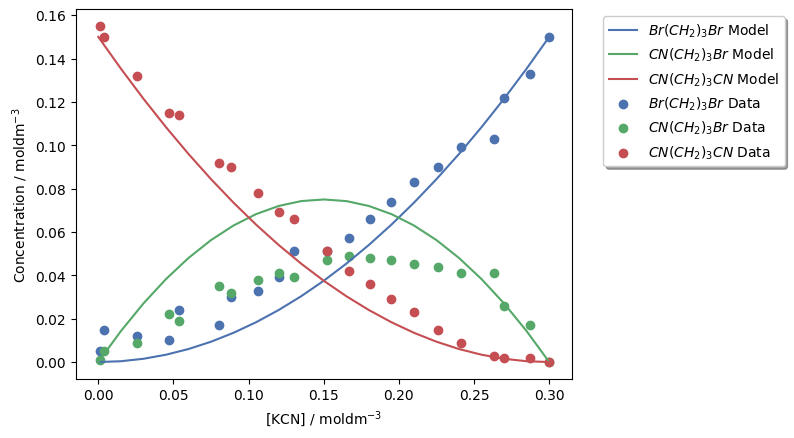
\includegraphics[width=0.8\linewidth]{PartA_Plot.png}
    \caption{A plot comparing the analytically modelled concentrations of species in solution compared to experimentally determined data.}
    \label{fig:Plot_A}
\end{figure}
Overall, the plotted experimental data and model data match moderately well - the overall mean squared error was 0.017. Visually, the $\ce{CN(CH2)3Br}$ model and data appear to have the worst discrepancy. This could be due to the simplifying assumption of $k_1 = 2k_2$, which does not account for the effect of the presence of the $\ce{CN-}$ group on the molecule compared to the $\ce{Br-}$ group - they have different electronegativities and group sizes for example, which will have steric and electronic effects on the molecule and its reactivity. An additional factor is possible error in calculations or code.

\section{Numerical Analysis}
\label{sec:Numerical}
\subsection{Generating the Numerical Model}
\begin{multicols}{2}
1. $\Delta[A] = -\frac{k_1[A]}{k_1[A] + k_2[C]}\Delta[B]_\text{cons}$\\
2. $\Delta[A] = -\frac{[A]}{[A]+K[C]}\Delta[B]_\text{cons}$\\
3. 
\begin{align*}
    \frac{\Delta[D]}{\Delta{t}}\times\frac{\Delta{t}}{\Delta[B]_\text{cons}} &= -\frac{k_2[B][C]}{k_1[A][B] - k_2[B][C]}\\
    \Delta{D} &= -\frac{k_2[C]}{k_1[A]-k_2[C]}\Delta[B]_\text{cons}
\end{align*}
4.
\begin{align*}
    [A]_0 &= [A] + [C] + [D]\\
    \Delta[A] &= [A] - [A]_0\\
    \Delta[C] &= [C]\\
    \Delta[D] &= [D]\\
    0 &= [A] - [A]_0 + [C] + [D]\\
    0 &= \Delta[A] + \Delta[C] + \Delta[D]\\
    \Delta[C] &= -\Delta[A] - \Delta[D]
\end{align*}
\end{multicols}
\subsection{Analysis of the Numerical Model with Python}
When the same assumption is used as section \ref{sec:Numerical}, with $K=0.5$, a slightly different plot is generated due to the way in which the relationships between species are modelled. In the analytical model, major simplifications were made about the relationship between the two rate constants, whereas in the numerical model, no such assumptions were made. This means that the numerical model should theoretically be much more accurate.
\begin{figure}[H]
    \centering
    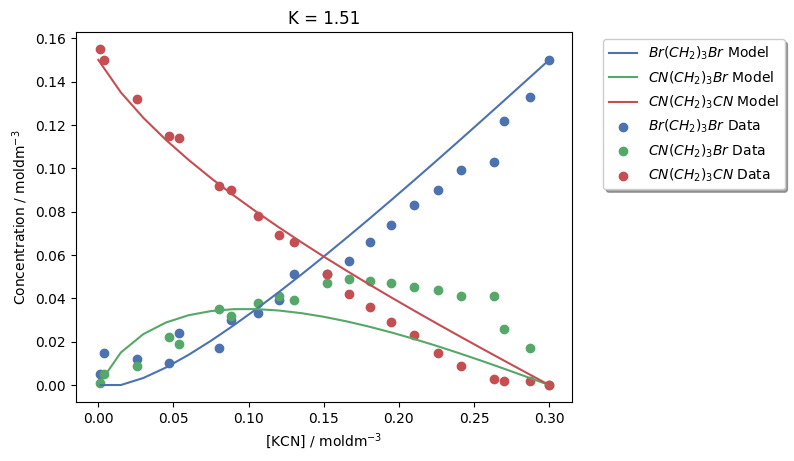
\includegraphics[width=0.8\linewidth]{PartB_Plot.png}
    \caption{A plot comparing the numerically modelled concentrations of species in solution compared to experimentally determined data.}
    \label{fig:Plot_B}
\end{figure}
In comparison to Fig. \ref{fig:Plot_A}, the fit of the model appears much closer to the experimental data. Additionally, the mean squared error was slightly lower. Compared to the analytical model, the K value is much higher ($\approx 3$ times). However, the model is still not a perfect fit to the experimental data. This is to be expected, as there are visually outliers in the experimental data, e.g. the $\ce{CN(CH2)3Br}$ point at $\sim$ 0.26 $\ce{[KCN]}$ mol dm$^{-3}$. Additionally, no model is perfect - they cannot account for every possible factor that can affect the rate of equation, e.g. stirring, temperature, etc.
\section{Appendix}
\begin{figure}[H]
    \centering 
    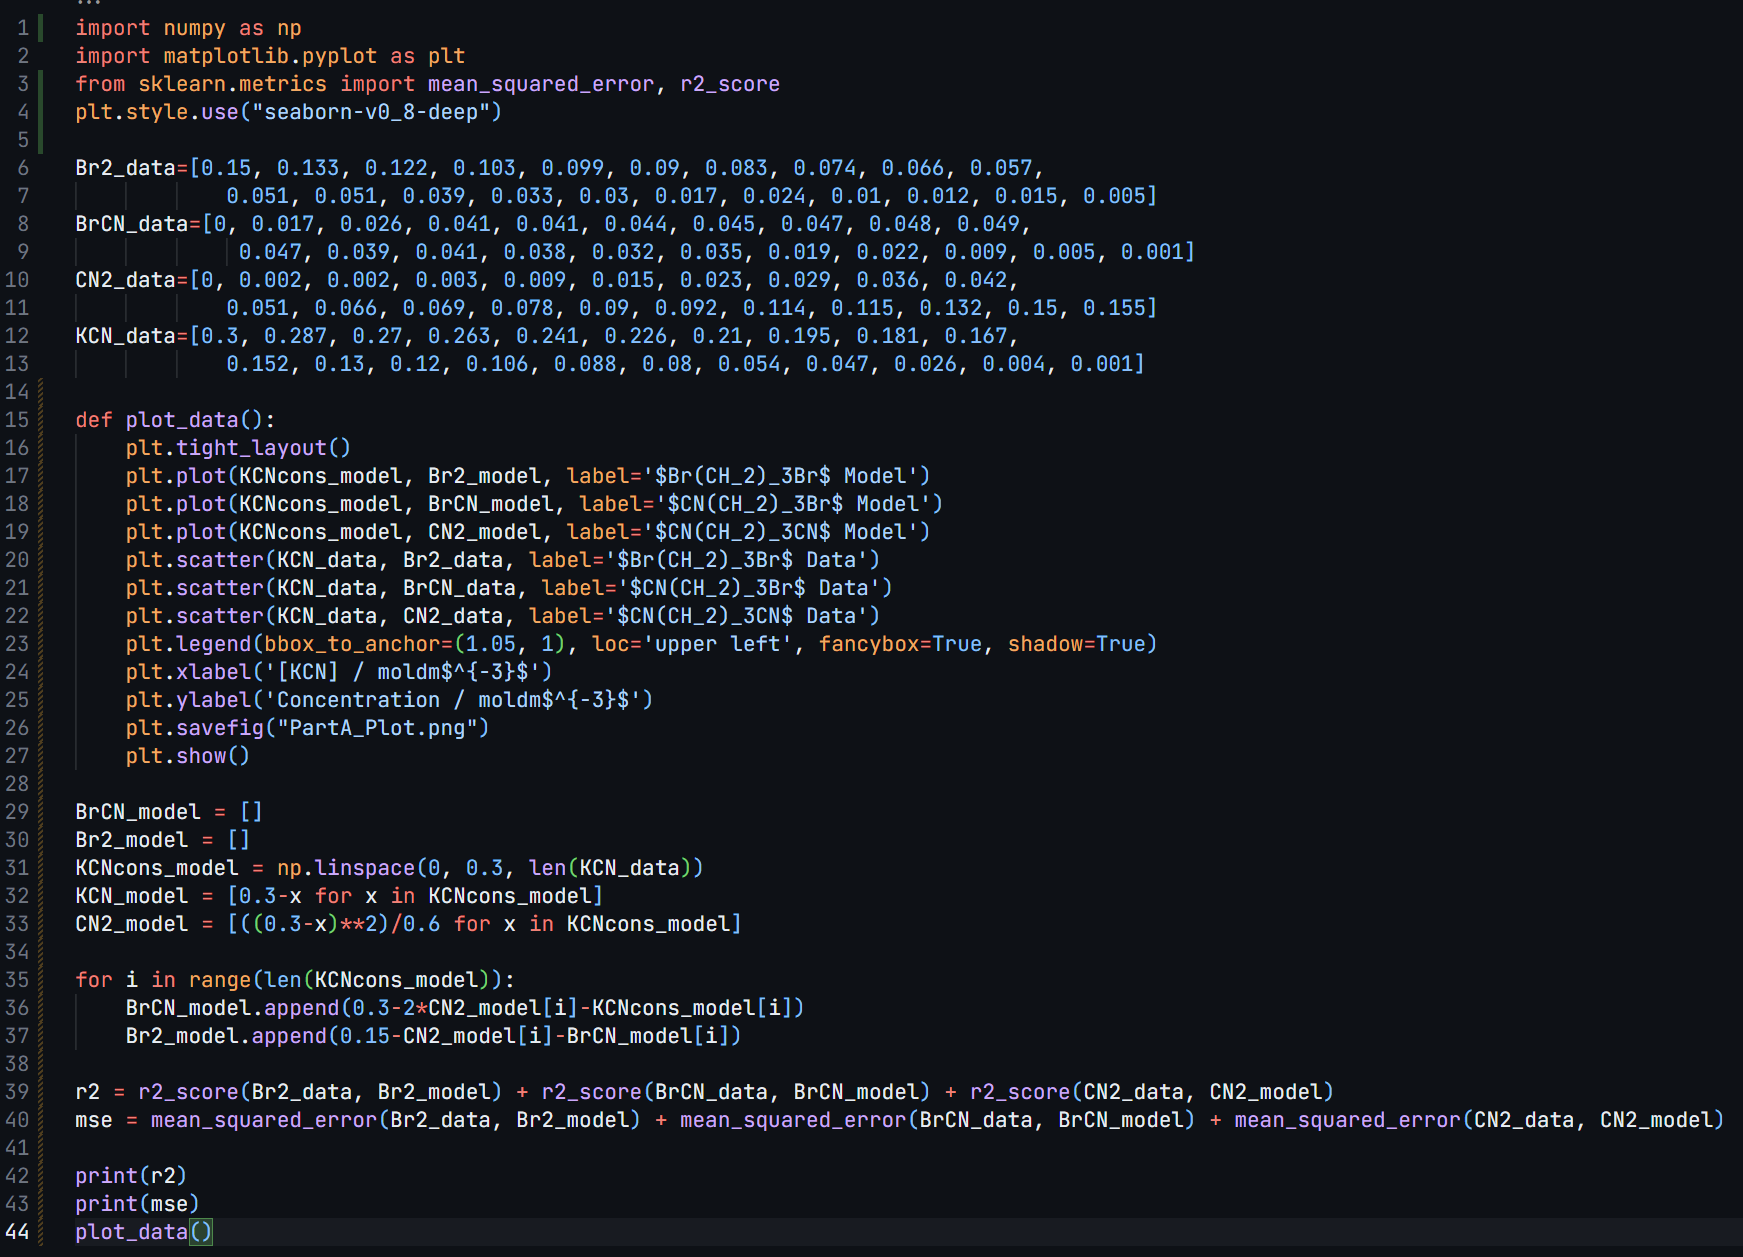
\includegraphics[width=0.9\linewidth]{PartA.png}
    \caption{The python code used for part A.}
\end{figure}
\bibliography{LabReport}
\bibliographystyle{rsc}
\end{document}